\documentclass[../../full]{subfiles}


\begin{document}
    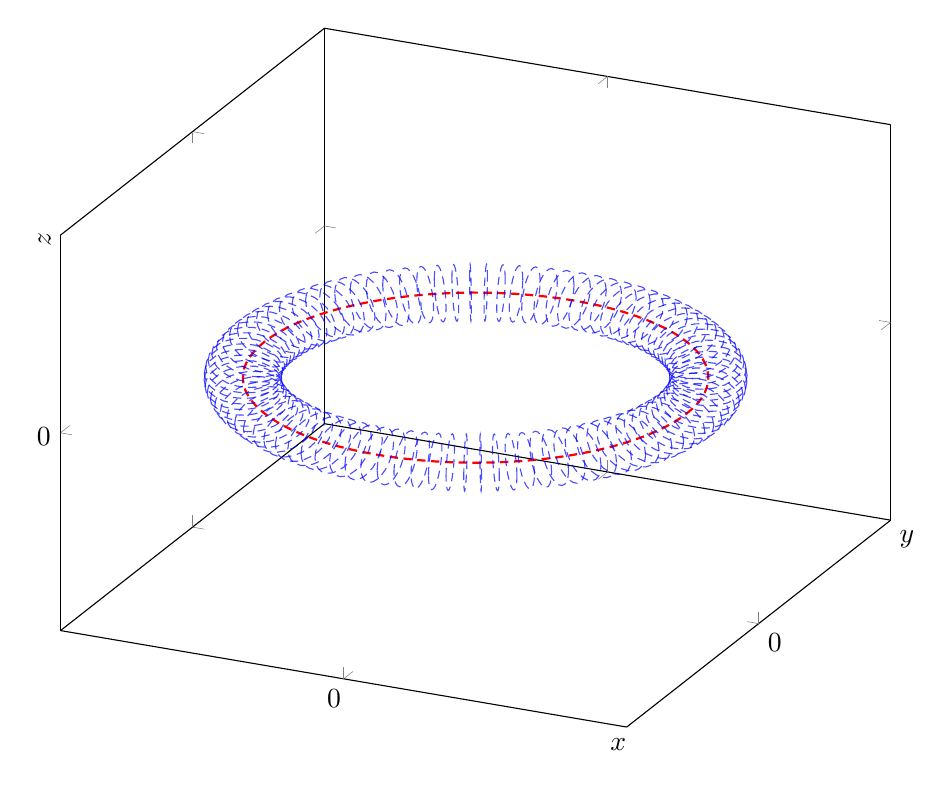
\begin{tikzpicture}
        % colors
        \def\ColorOrigin{Red}
        \def\ColorWire{Blue}
        % angles
        \def\AnglePartsOrigin{96}
        \def\AnglePartsWire{24}
        % Radius
        \def\RLarge{6}
        \def\RSmall{1}
        \pgfmathtruncatemacro\RMax{\RLarge+\RSmall}
        %
        \begin{axis}[
            width=\textwidth,
            view={25}{30},
            xlabel={\( x \)},
            ylabel={\( y \)},
            zlabel={\( z \)},
            xmin=-\RMax, xmax=\RMax,
            xtick={0},
            ymin=-\RMax, ymax=\RMax,
            ytick={0},
            zmin=-\RMax, zmax=\RMax,
            ztick={0},
            enlargelimits=0.075,
            every axis x label/.append style={at=(ticklabel* cs:1)},
            every axis y label/.append style={at=(ticklabel* cs:1)},
            every axis z label/.append style={at=(ticklabel* cs:1)},
        ]
            % origin path
            \def\OriginPath{}
            \foreach \i [
                    evaluate=\i as \AnglePhi
                                using (360/\AnglePartsOrigin*\i),
                    evaluate=\AnglePhi as \Ox
                                using (\RLarge*cos(\AnglePhi)),
                    evaluate=\AnglePhi as \Oy
                                using (\RLarge*sin(\AnglePhi)),
            ] in {0, ..., \AnglePartsOrigin} {
                \global\edef\OriginPath{\OriginPath (\Ox, \Oy, 0)}
            }
            \addplot3 [\ColorOrigin, no marks, thick, densely dashed]
                coordinates { \OriginPath };
            % Wireframe shape
            \foreach \i [
                    evaluate=\i as \AnglePhi
                                using (360/\AnglePartsOrigin*\i),
                    evaluate=\AnglePhi as \Ox
                                using (\RLarge*cos(\AnglePhi)),
                    evaluate=\AnglePhi as \Oy
                                using (\RLarge*sin(\AnglePhi)),
            ] in {1, ..., \AnglePartsOrigin} {
                \def\temp{}
                \foreach \j [
                        evaluate=\j as \AnglePsi
                                    using (360/\AnglePartsWire*\j),
                        evaluate=\AnglePsi as \Px
                                    using (\Ox + \RSmall*cos(\AnglePsi)*cos(\AnglePhi)),
                        evaluate=\AnglePsi as \Py
                                    using (\Oy + \RSmall*cos(\AnglePsi)*sin(\AnglePhi)),
                        evaluate=\AnglePsi as \Pz
                                    using (\RSmall*sin(\AnglePsi)),
                ] in {0, ..., \AnglePartsWire} {
                    \global\edef\temp{\temp (\Px, \Py, \Pz)}
                }
                \edef\temp{
                    \noexpand \addplot3
                        [\ColorWire, no marks, densely dashed, opacity=0.7]
                        coordinates {\temp};
                }
                \temp
            }
        \end{axis}
    \end{tikzpicture}
\end{document}
